\subsection{Recurrent Neural Networks \cite{olah2015} \cite{salamon2020}}
One fundamental aspect of human cognition is the ability to leverage context when processing information. We understand each word in a sentence not in isolation but concerning those preceding it. Similarly, our comprehension of a movie scene hinges on the accumulated understanding of prior scenes. This inherent "persistence of thought" poses a significant challenge for traditional neural networks, which operate on independent snapshots of data. Their static architecture struggles to incorporate temporal dependencies, hindering their ability to learn from sequential data.

Consider the task of classifying events in a film sequence. A conventional neural network analyzing each frame individually would lack the capacity to recognize overarching themes or draw connections across scenes. This shortcoming arises from the network's inability to store and utilize memory, leading to fragmented and context-agnostic interpretations.

Recurrent neural networks (RNNs) overcome this limitation by introducing internal loops that enable information persistence. Unlike their static counterparts, RNNs possess the ability to retain and integrate relevant information from previous input steps, allowing them to build a dynamic understanding of sequences.

This internal memory mechanism can be visualized through the concept of hidden states. As depicted in Figure \ref{fig:rnn}, part of the network (denoted by "A") processes an input $x_t$ and generates an output $h_t$. Crucially, a loop feeds this output back into the network at the next timestep, allowing it to influence the processing of subsequent inputs. In essence, this creates a chain reaction where each step carries forward the accumulated knowledge from previous iterations.

Thinking of an RNN as a chain of interconnected modules clarifies this concept further. Each module receives information from its predecessor, processes it based on its internal state (influenced by past inputs), and generates its output to be passed on. This "message-passing" mechanism allows the network to build a holistic understanding of the sequence by progressively incorporating context with each step.

The inherent memory capability of RNNs makes them uniquely suited for tasks involving sequential data. They excel in applications like language processing, where understanding sentence structure and semantics requires considering the order of words; speech recognition, where capturing the nuances of spoken language hinges on temporal context; and time series analysis, where predicting future values based on past trends necessitates memory of previous data points.

\begin{figure} [H]
    \centering
    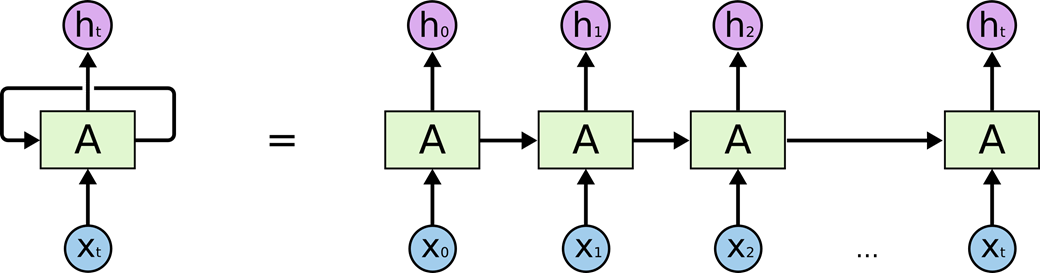
\includegraphics[width=0.75\linewidth]{images/dl/rnn.png}
    \caption{On the left, the looped version of a recurrent layer. On the right, is the unrolled equivalent version of a recurrent layer.}
    \label{fig:rnn}
\end{figure}
